\chapter{Simulating anisotropic diffusion in heterogeneous brain regions}
\label{chp:chp6}


In this chapter, we bring together the different tools and techniques, discussed 
throughout the text, to perform a comprehensive simulation of the following 
continuous problem
\begin{align}\label{eqn:chp6:model-problem}
	\partial_t u = \Div\left(\tnsr{K(x)} \Grad u\right) + f,& \quad x\in\Omega \text{ and } t>0,\\
	u=u_d(t,x),&\quad x\in\partial\Omega \text{ and } t>0, \\ 
        u(0,x) =  u_0(x),&\quad x\in \Omega \text{ and } t=0.
\end{align}
The computational mesh, $\Omega_h$, is determined from T1 data and is  
divided into grey and white matter subdomains; DTI data is employed in the 
construction of the diffusion tensor, $K(x)$, and select specific  
sub-regions, such as the hippocampus, will be selected to assess site-specific 
clearance.  For a point $x$ in the gray matter, $K(x)$ is known to be isotropic and can 
therefore be approximated by a scalar.  In the grey matter, the mean values of 
the apparent diffusion coefficient of water in young and healthy subjects is known 
to in the range of $0.78-1.09 \times 10^{-3} \mbox{mm}^2 /\mbox{s}$.  In the white 
matter, $K(x)$ is anisotropic and is represented as a symmetric, positive definite 
$3\times 3$ matrix with an apparent diffusion coefficient in the range of 
$0.7-0.9 \times 10^{-3}\mbox{mm}^2/\mbox{s}$ (c.f.~\cite{helenius2002diffusion}). 

In practice, one must first address data and mesh-resolution issues 
informing $K(x)$ and $\Omega_h$.  For instance, raw diffusion tensor data can exhibit 
a certain degree of sharp, or rough, transitions in addition to noise; 
c.f.~Fig~\ref{fig:chp5:freesurfer-parc}.  This is particularly true in the grey 
matter proximal to the cerebrospinal fluid.  Here, we assume that the DTI data 
has been suitably smoothed, and de-noised, for use in simulations.  In addition, 
we must contend with the critical question of ascertaining a suitable mesh resolution; 
this consideration directly impacts the computational costs and results.
A resolution which is suitable to provide reliable estimates of the clearance, 
or spread, of molecules of difference sizes is essential; however, we also seek 
to avoid over-resolving the mesh to avoid incurring an unnecessary computational 
costs.  

%\kent{In the 3D simulations we actually do not estimate clearance but rather 
%the spread of Amyloid beta from CSF and into the brain. I think I have read that 
%Amyloid-beta in CSF vary during day-night. But it might be that Amyloid goes 
%from brain to CSF rather than the other way. }
%\kent{Hippocampus or hippocampus}
%\tbt{hippocampus, it is an anatomical region and not a proper noun}

%\section{Clearance in a 1D brain}\label{sec:chp6:1D-tests}
\section{Molecular diffusion in 1D}\label{sec:chp6:1D-tests}
In order to estimate the required spatial mesh resolution, discrete time step, 
and the time scale of solute clearance, it is useful to consider 
\eqref{eqn:chp6:model-problem} in one dimension.  Molecules of different sizes 
are also considered; in particular, Amyloid-beta, the tracer Gadovist, and water.  
The effective diffusion constant, $D$, for these three molecules are estimated to 
be $6.2e-5 \mbox{mm}^2/\mbox{s}$, $1.3e-4 \mbox{mm}^2/\mbox{s}$ and 
$1.1e-3 \mbox{mm}^2/\mbox{s}$, respectively~\cite{waters2010concentration,valnes2020apparent}. 
In one dimension, the parabolic diffusion problem \eqref{eqn:chp6:model-problem} 
admits a simple analytic solution for the initial and boundary conditions 
$u_0(x)=0$, $u(0,t)=1$ and $u(\infty,t)=0$.  The analytic solution is 
\begin{equation}
\label{analytical:1D}
u(x,t) =  \mbox{erfc}(x / (2 \sqrt{D t})),
\end{equation}
and a plot of \eqref{analytical:1D} appears in Figure~\ref{fig:chp6:analytics} 
for a 2mm slice (left) and 1cm slice (middle), after 9 hours, alongside a 1cm slice 
after 24 hours (right).  It is evident, from Figure~\ref{fig:chp6:analytics}, that 
diffusion is a slow process.  Figure~\ref{fig:chp6:analytics} (left) shows that 
significant clearance occurs within 2mm of the boundary at the nine hour time point; 
however, 1cm away it is observed that the heavier molecules, Amyloid-beta and Gadovist, 
have concentrations near zero.  
\begin{figure}	
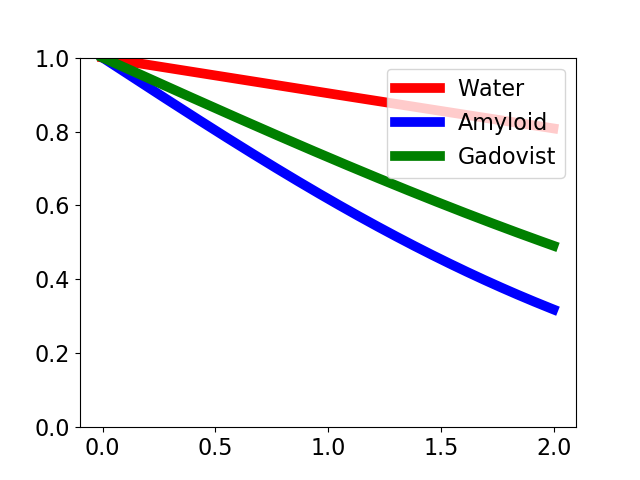
\includegraphics[width=0.32\textwidth]{./chapters/chp6/FIG/9hours_2mm_WAG}
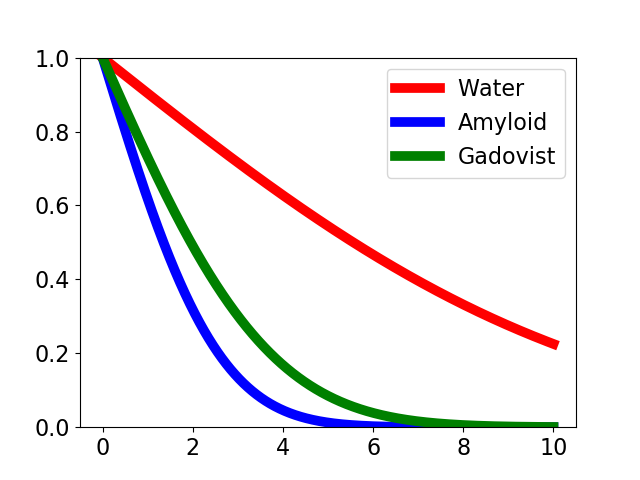
\includegraphics[width=0.32\textwidth]{./chapters/chp6/FIG/9hours_1cm_WAG}
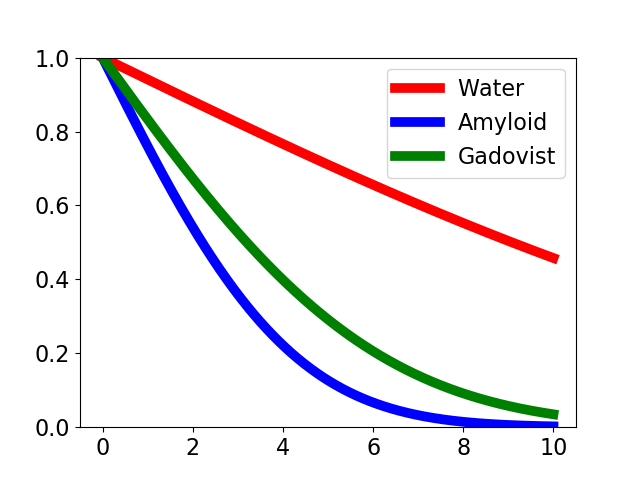
\includegraphics[width=0.32\textwidth]{./chapters/chp6/FIG/24hours_1cm_WAG}
\caption{
Diffusion %of Amyloid-beta, Gadovist and water 
according to \eqref{analytical:1D}; concentration (y-axis) 
versus distance (x-axis). Concentration in a 2mm slice (left) and 1cm slice (middle) after 9 hours and 
in a 1cm slice (right) after 24 hours. 
}
\label{fig:chp6:analytics}
\end{figure}
%\kent{axis font and legend ok or too small?}
%\tbt{they are ok}

Equation \eqref{eqn:chp6:model-problem} is then discretized using the finite element 
approach discussed in Chapter~\ref{chp:chp3}.  The source code for the one-dimensional 
analytic solution \eqref{analytical:1D} and one-dimensional discretization of  
\eqref{eqn:chp6:model-problem} are provided, in full, in the files \emp{analytical\_1D.py} 
and \emp{diffusion\_1D.py}, respectively.  The sharp change in the boundary-versus-initial 
conditions for our model problem can lead to numerical oscillations in the finite element 
solution when using the standard Galerkin method, as discussed in Chapter~\ref{chp:chp3}.  
Such oscillations diminish with refinement; they can also be avoided through the use of 
so-called monotonic or maximum principle preserving schemes.  Another common method, 
that we consider here, for Galerkin finite element schemes is called mass lumping.

Figures \ref{fig:chp6:numerics1} and \ref{fig:chp6:numerics2} depict the standard 
Galerkin solution and mass-lumped Galerkin solution, respectively, for different 
configurations.  Figure \ref{fig:chp6:numerics1} shows the distribution of Amyloid-beta 
in a 5cm slice, after 30 minutes, using the standard (left) and mass-lumped (right) 
Galerkin approach; for coarse resolutions (N=10 or N=20) the standard approach (left) 
yields considerable non-physical oscillations while the mass-lumped solution (right) 
produces significant numerical diffusion.  Figure \ref{fig:chp6:numerics2} shows the 
long-term diffusive behaviour, over nine hours, in a 5mm slice.  In the long-term 
context, the Galerkin scheme (Figure~\ref{fig:chp6:numerics2}, left) is clearly 
desirable when contrasted with the overly-diffusive mass-lumped Galerkin 
approach (Figure~\ref{fig:chp6:numerics2}, right); the former allows for a spatial 
resolution of $N=10$ or $N=20$ while the latter requires $N=40$ or $N=80$ to control 
the numerical diffusion.  Essentially, the initial error from the short-term Gibbs 
phenomena, from the discontinuous initial data, in Figure~\ref{fig:chp6:numerics1} (left) 
is no match for the long-term regularizing effect of the parabolic PDE 
\eqref{eqn:chp6:model-problem}; thus, these early errors do not contribute much 
to the long-term numerical solution.  

The results of Figures~\ref{fig:chp6:numerics1} and \ref{fig:chp6:numerics2} suggest 
that, if we are interested in long-term dynamics, a time-step size of 
$\Delta t \approx 6/540$ with spatial resolution of $N=10$ or $N=20$, corresponding 
roughly to a quasi-uniform mesh simplicial diameter of $0.25 \mbox{mm} \leq h \leq 0.5 \mbox{mm}$, is 
a good starting target for the standard Galerkin approach in our 3D discretization.  
Conversely, a mesh size of $N=80$, or $h\approx 6.25\times 10^{-2}\mbox{mm}$, is needed 
for the mass-lumped case; this would be a much more costly choice on a 3D 
mesh if the short term dynamics, of Figure~\ref{fig:chp6:numerics1}, need not be 
resolved. 


\begin{figure}	
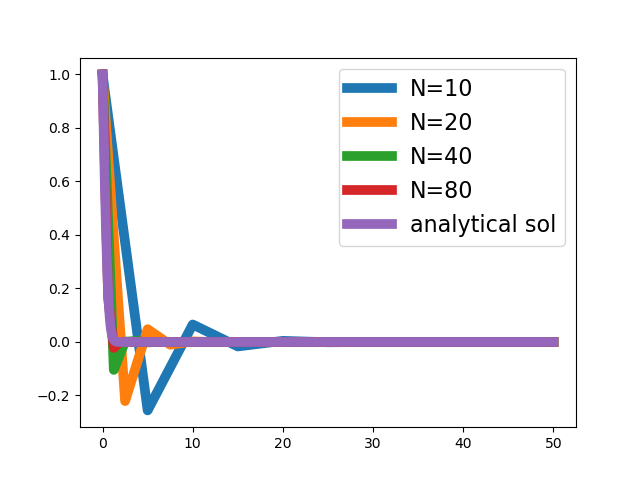
\includegraphics[width=0.49\textwidth]{./chapters/chp6/FIG/Amyloid_numerical_1D_L_max50_dt300_final1800_lumpednot.png}
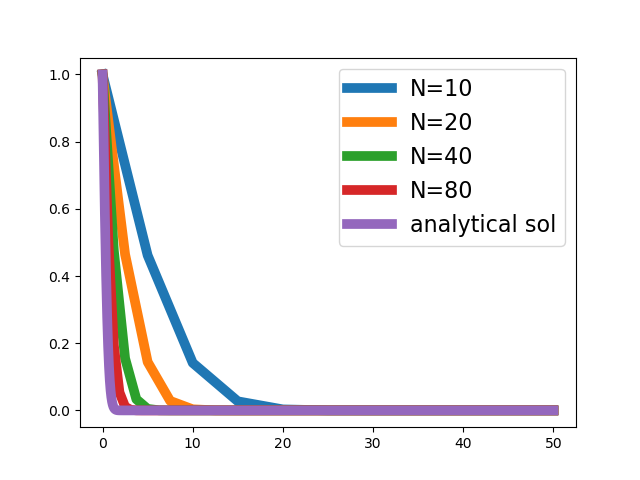
\includegraphics[width=0.49\textwidth]{./chapters/chp6/FIG/Amyloid_numerical_1D_L_max50_dt300_final1800_lumpedlumped.png}
\caption{
%Distribution of Amyloid-beta over 5 cm at different after 30 minutes with time step of 6 minutes are shown in the left 
%and right figure, respectively. The leftmost picture shows a standard Galerkin scheme, while a lumped mass matrix is used
%for the rightmost illustration.
Solution of \eqref{eqn:chp6:model-problem} over a 5cm slice, final time T=30 min and $\Delta t = 6/30$. 
Amyloid-beta concentration (y-axis) v.s.~length (x-axis). Standard Galerkin (left) and mass-lumped 
Galerkin (right) discrete schemes. 
}
\label{fig:chp6:numerics1}
\end{figure}

\begin{figure}	
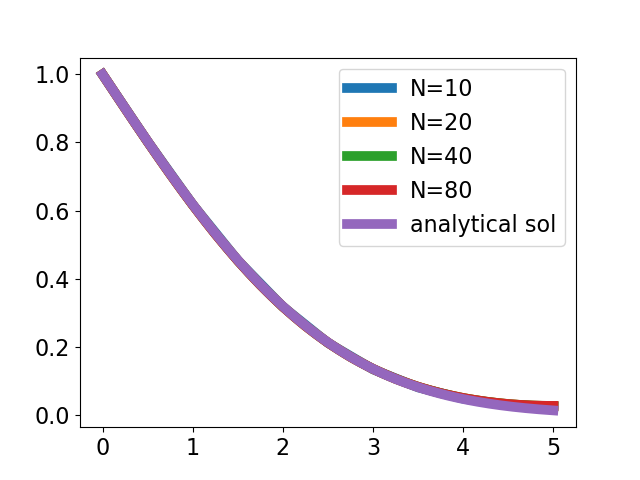
\includegraphics[width=0.49\textwidth]{./chapters/chp6/FIG/Amyloid_numerical_1D_L_max5_dt300_final32400_lumpednot.png}
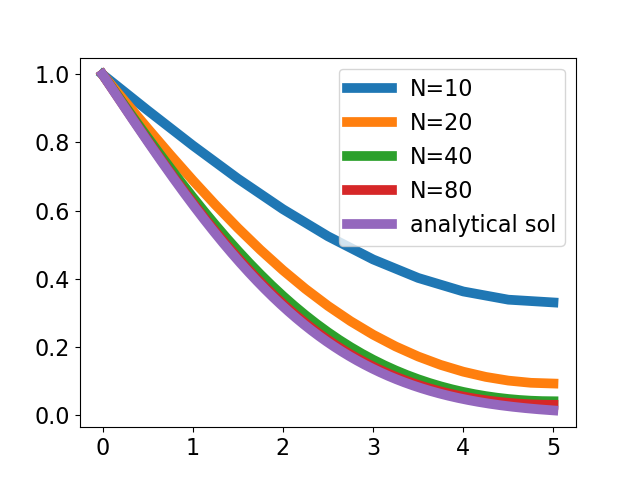
\includegraphics[width=0.49\textwidth]{./chapters/chp6/FIG/Amyloid_numerical_1D_L_max5_dt300_final32400_lumpedlumped.png}
\caption{
%Distribution of Amyloid-beta over 5 mm at different after 9 hours with time step of 6 minutes are shown in the left 
%and right figure, respectively. The leftmost picture shows a standard Galerkin scheme, while a lumped mass matrix is used
%for the rightmost illustration.
Solution of \eqref{eqn:chp6:model-problem} over a 5cm slice, final time T=9h and $\Delta t = 6/540$. 
Amyloid-beta concentration (y-axis) v.s.~length (x-axis). Standard Galerkin (left) and mass-lumped 
Galerkin (right) discrete schemes. 
}
\label{fig:chp6:numerics2}
\end{figure}



%\section{Estimating clearance rate in selected regions, with DTI}\label{sec:chp6:3D}
\section[Estimating regional anisotropic Amyloid-beta diffusion ]{Estimating regional anisotropic Amyloid-beta diffusion with DTI in a 3D brain domain}\label{sec:chp6:3D}
In this section we consider simulations involving Amyloid-beta.  As the molecule 
with lowest apparent molecular diffusivity, Amyloid-beta is the most difficult 
to simulate numerically.  
\begin{lstlisting}[style=bashStyle]
# convert mesh to h5 file 
python3 3D_to_FEniCS.py Mesh_16.mesh Mesh_16.h5

# add markers for hippocampus, insula, superiorfrontal 
python3 add_parcellations.py --parc wmparc.mgz \ 
  --in_mesh Mesh_16.h5 --out_mesh Mesh_parc_16.h5 \ 
  --add 17 1028 1035 253 3028 3035    

# add dti to the h5 file. 
python3 dti_data_to_mesh.py  --dti preped_tensor.mgz \
  --mesh Mesh_parc_16.h5 --label 1 0.4 0.6 \ 
  --out DTI_16.h5 

# run simulation  
python3 chp6-diffusion-mritracer.py \ 
  --mesh DTI_16.h5 \ 
  --lumped lumped --label=DTI16lumped 
\end{lstlisting}

\begin{python}

# read mesh, subdomains and tensor  
mesh = Mesh()
hdf = HDF5File(mesh.mpi_comm(),args.mesh, "r")
hdf.read(mesh, "/mesh", False)  
subdomains = MeshFunction("size_t", mesh, mesh.topology().dim())
hdf.read(subdomains, "/subdomains")
boundaries  = MeshFunction("size_t", mesh, mesh.topology().dim() - 1)
hdf.read(boundaries, "/boundaries")
dx = Measure("dx", domain=mesh, subdomain_data=subdomains)
ds = Measure("ds", domain=mesh, subdomain_data=boundaries)
T = TensorFunctionSpace(mesh, "DG",0)
Kt = Function(T) 
hdf.read(Kt, "/DTI")


# the weak form of the equation  
# notice that the diffusion tensor K is only used in 
# the white matter (2, 3028, 3035)   	
F = mass_form = v*u*dx \
    dt*D_scale*MD_grey*dot(grad(u), grad(v))*dx(1)+ \  
    dt*D_scale*MD_grey*dot(grad(u), grad(v))*dx(17) +  
    dt*D_scale*MD_grey*dot(grad(u), grad(v))*dx(1035) + \ 
    dt*D_scale*MD_grey*dot(grad(u), grad(v))*dx(1028) - \
    dt*D_scale*dot(grad(u), dot(Kt, grad(v)))*dx(2)  + \
    dt*D_scale*dot(grad(u), dot(Kt, grad(v)))*dx(3028) +\ 
    dt*D_scale*dot(grad(u), dot(Kt, grad(v)))*dx(3035) +\ 
    (u_n + dt*f)*v*dx

a, L = lhs(F), rhs(F)

t = 0

time_points = []
for n in range(time_steps):
    t += dt
    b = assemble(L)
    bc.apply(A,b)
    solve(A,u.vector(),b, "gmres", "amg")

    # write a visualization file result for every hour 
    if t/(60*60) - int(t/(60*60)) < dt/(60*60):  vtkfile << (u, t)
    u_n.assign(u)

    #calculate the average concentration of the different subdomains
    unit17 += [assemble(u*dx(17))/vol17]
    unit1035 += [assemble(u*dx(1035))/vol1035]
    unit1028 += [assemble(u*dx(1028))/vol1028]
    unit3028 += [assemble(u*dx(3028))/vol3028]
    unit3035 += [assemble(u*dx(3035))/vol3035]
    time_points += [t] 
\end{python}
\tbt{@Kent: The boundary conditions `bc' are used in the time loop but othewise undefined in the script above. 
It also appears that you are missing A=assemble(a). dt is also undefined. time\_steps is 
also undefined.  These issues should be rectified or the user should be informed that 
the above is a code snippet (for illustration) and that the corresponding code can 
be found in `somefilename.py' in the corresponding chapter source directory.}

Pursuant to the observations of Section~\ref{sec:chp6:1D-tests}, equation 
\eqref{eqn:chp6:model-problem} is solved, on the 3D brain mesh with SVMTK 
resolution $64$ using FEniCS, in the code above for a time course of 9 hours 
and $\Delta t = 6/580$ using the standard Galerkin method. Average concentrations 
are computed for regions 17 (hippocampus), 1035 (insula grey matter), 3035 
(insula white matter), 1028 (superiorfrontal grey matter), and 3028 
(superiofrontal white matter); the resulting average concentration plot is shown 
in Figure \ref{chp6:regions}. In contrast to the plots in Section~\ref{sec:chp6:1D-tests},  
we here consider the tracer distribution in certain regions as a function of 
time; they therefore start at a low value and increase with time as Amyloid-beta 
diffuses throughout the brain. 

Figure~\ref{chp6:regions} makes clear that the distribution of Amyloid-beta 
in the grey matter regions and Hippocampus are affected much more than in the 
white matter regions; this expected due to the fact that both the grey matter 
and hippocampus are closer to the CSF where, in our simulation, the Amyloid-beta 
concentration is assumed to reside initially.  It is also observed that the 
`top' regions,  i.e. the superiorfrontal grey and white matter (1028 and 3028 
respectively), experience faster Amyloid-beta deposition than the corresponding 
regions on the side of the brain.  
\begin{figure}	
\centering
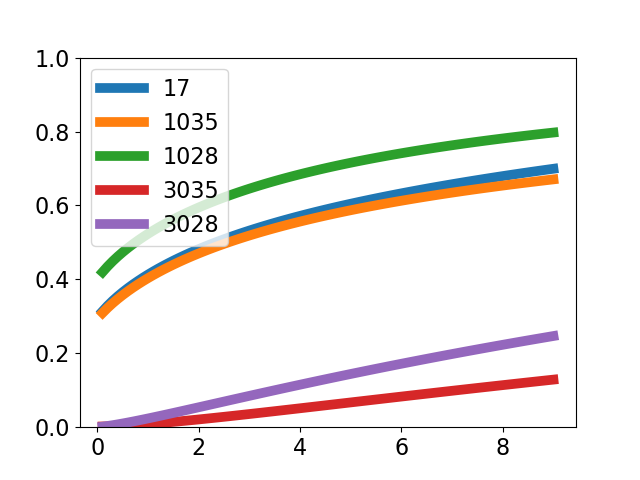
\includegraphics[width=0.7\textwidth]{./chapters/chp6/FIG/tracer_uniform_notlump_regions_64.png}
\caption{
%Distribution of Amyloid-beta in the regions Hippocampus (17), insula (grey matter:1035, white matter: 3035), superiorfrontal (grey matter: 1028 and white matter: 3028)  
%during 9 hours with time step of 6 minutes are shown when using standard Galerkin method in the 64 mesh. 
Amyloid-beta concentration (y-axis) versus time (x-axis) in hours. 
}
\label{chp6:regions}
\end{figure}

It is important to note, though, that we have not yet computationally 
established mesh convergence; thus, one should avoid drawing any final conclusions 
from this initial demonstration.  Next, we investigate the mesh convergence of 
the standard Galerkin and mass-lumped Galerkin approaches.  In this set of examples 
we consider a roughly uniform refinement, but the mesh is actually not refined in 
place; rather, a sequence of meshes is first generated at different resolutions 
using SVMTK. That is, we construct a sequence of quasi-uniform meshes as follows: 
\begin{python}
import SVMTK as svm
import numpy as np
import time

mesh_dir="../PROCESSED-DATA/KENT/mesh/"
print(mesh_dir+"new-vent.off") 
vent  = svm.Surface(mesh_dir+"new-vent.off") 
lhpial = svm.Surface(mesh_dir+"lh-pial-new.off") 
rhpial = svm.Surface(mesh_dir+"rh-pial-new.off") 
white  = svm.Surface(mesh_dir+"new-white.off") 

smap = svm.SubdomainMap() 
smap.add("1000",1)
smap.add("0100",1) 
smap.add("0110",2)
smap.add("0010",2)
smap.add("1010",2)
smap.add("0111",3)
smap.add("1011",3)

surfaces = [lhpial,rhpial,white,vent] 

domain = svm.Domain(surfaces,smap)

Ns = [16,32,64,128]
for N in Ns: 
    t0 = time.time()
    domain.create_mesh(N) 
    domain.remove_subdomain([3]) 
    domain.save("Mesh_\%d.mesh" \% N)
\end{python}
Mesh convergence results, for the mesh sequence generated above, are shown in 
Figure~\ref{fig:chp6:numerics2}; it is clear that the standard Galerkin approach 
(Figure~\ref{fig:chp6:numerics2} left) outperforms that of the the mass-lumped 
Galerkin scheme.   However, even for standard Galerkin scheme, the convergence 
seems questionable at the highest resolution tested (around 15.5M simplicial 
elements).  Recall that piecewise constant discontinuous Galerkin elements are 
used to construct the anisotropic DTI tensor, $K(x)$.  This DG construction 
requires around 140 million values (i.e. 9 entries per simplex, and 15.5M 
simplices) and higher resolution, such as those for piecewise linear or 
quadratic constructions, are not possible on a personal computing device with 
only 32 gigabytes of RAM.  Thus, we also assess mesh convergence by adaptively 
refining in a selected region.  Here, we focus on the hippocampus. 
%Hence, in order to assess the performance we addaptively refine in selected regions. In this example, 
%we focus on Hippocampus. 

Figure~\ref{fig:chp6:numerics3} shows the computational convergence pursuant to 
the use of adaptively refined meshes.  Using this technique, mesh convergence 
in the hippocampus has been obtained for the standard Galerkin scheme 
(Figure~\ref{fig:chp6:numerics3}, left) after two regional refinements.  However, 
mesh convergence for the the mass-lumped Galerkin strategy 
(Figure~\ref{fig:chp6:numerics3}, right) remains unclear; even after four 
refinements to the hippocampal region.  Tables~\ref{tab:uniref} 
and \ref{tab:localref} list the number of vertices, cells and the minimal and 
maximal mesh sizes for the uniform (Figure~\ref{fig:chp6:numerics2}) and 
adaptive (Figure~\ref{fig:chp6:numerics3}) strategies, respectively.  We see that 
the actual $h$ required for mesh convergence is around 2-10 times smaller than 
our initial estimate in 1D (Section~\ref{sec:chp6:1D-tests}) test 
case.  

\begin{figure}	
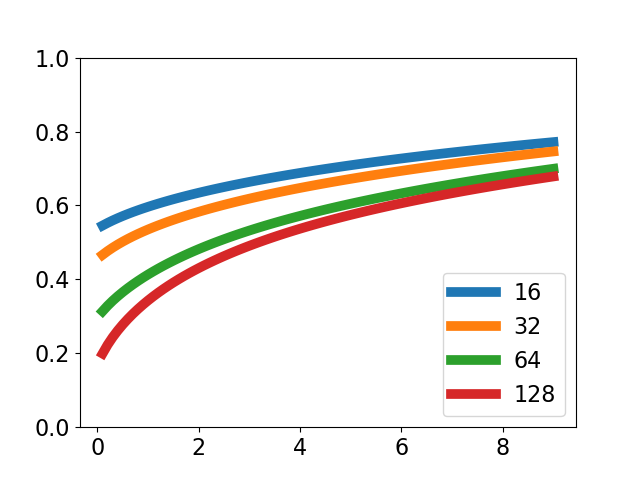
\includegraphics[width=0.49\textwidth]{./chapters/chp6/FIG/tracer_hippocampus_uniform_notlump.png}
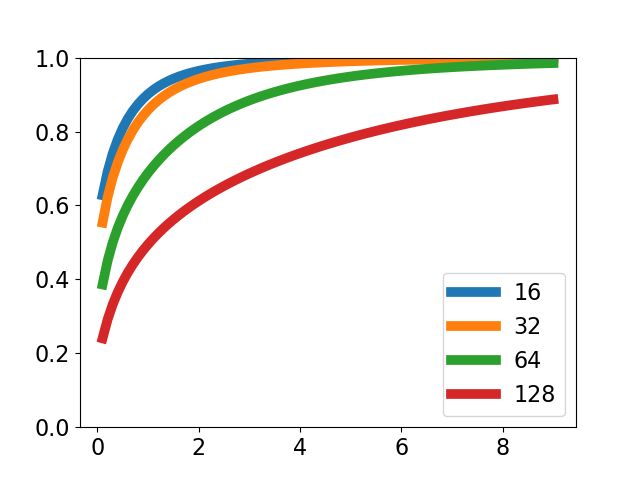
\includegraphics[width=0.49\textwidth]{./chapters/chp6/FIG/tracer_hippocampus_uniform_lump.png}
\caption{
%Distribution of Amyloid-beta over 5 mm in hippocampus during 9 hours with time step of 6 minutes are shown in the left 
%and right figure, respectively, when using a roughly uniform mesh size.  
%The leftmost picture shows a standard Galerkin scheme, while a lumped mass matrix is used
%for the rightmost illustration.
Amyloid-beta (y-axis) versus time (x-axis) in hours; 5mm hippocampal slice over 
9h, $\Delta t = 6/540$. Quasi-uniform mesh domain sequence, various resolutions, generated by SVMTK. 
Standard Galerkin (left) versus mass-lumped Galerkin (right) discretizations.
}
\label{fig:chp6:numerics2}
\end{figure}

\begin{figure}	
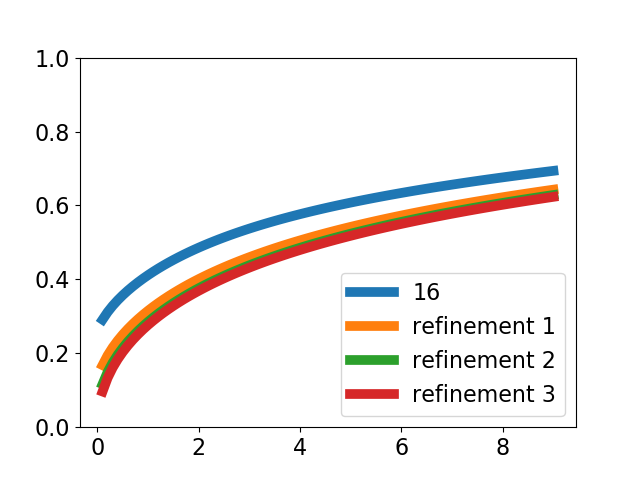
\includegraphics[width=0.49\textwidth]{./chapters/chp6/FIG/tracer_hippocampus_notlumped_addaptive.png}
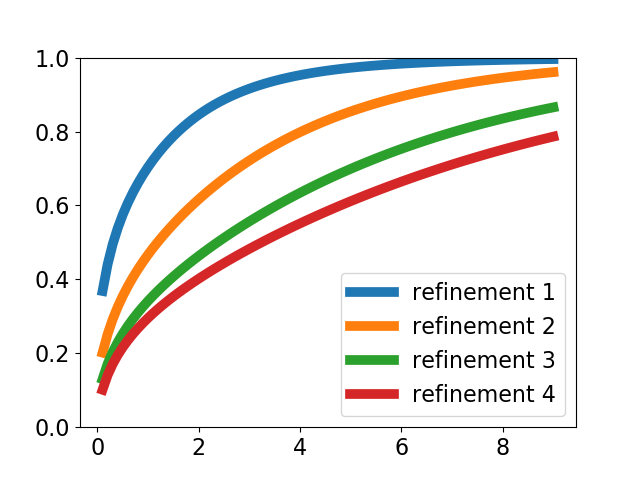
\includegraphics[width=0.49\textwidth]{./chapters/chp6/FIG/tracer_hippocampus_lumped_addaptive.png}
\caption{
%Distribution of Amyloid-beta over 5 mm in hippocampus during 9 hours with time step of 6 minutes are shown in the left 
%and right figure, respectively, when using local refinement in the hippocampus area.  
%The leftmost picture shows a standard Galerkin scheme, while a lumped mass matrix is used
%for the rightmost illustration.
Amyloid-beta (y-axis) versus time (x-axis) in hours; 5mm hippocampal slice over 
9h, $\Delta t = 6/540$. Adaptive hippocampal refinements.  Standard Galerkin (left) 
versus mass-lumped Galerkin (right) discretizations.
}
\label{fig:chp6:numerics3}
\end{figure}

\begin{figure}	
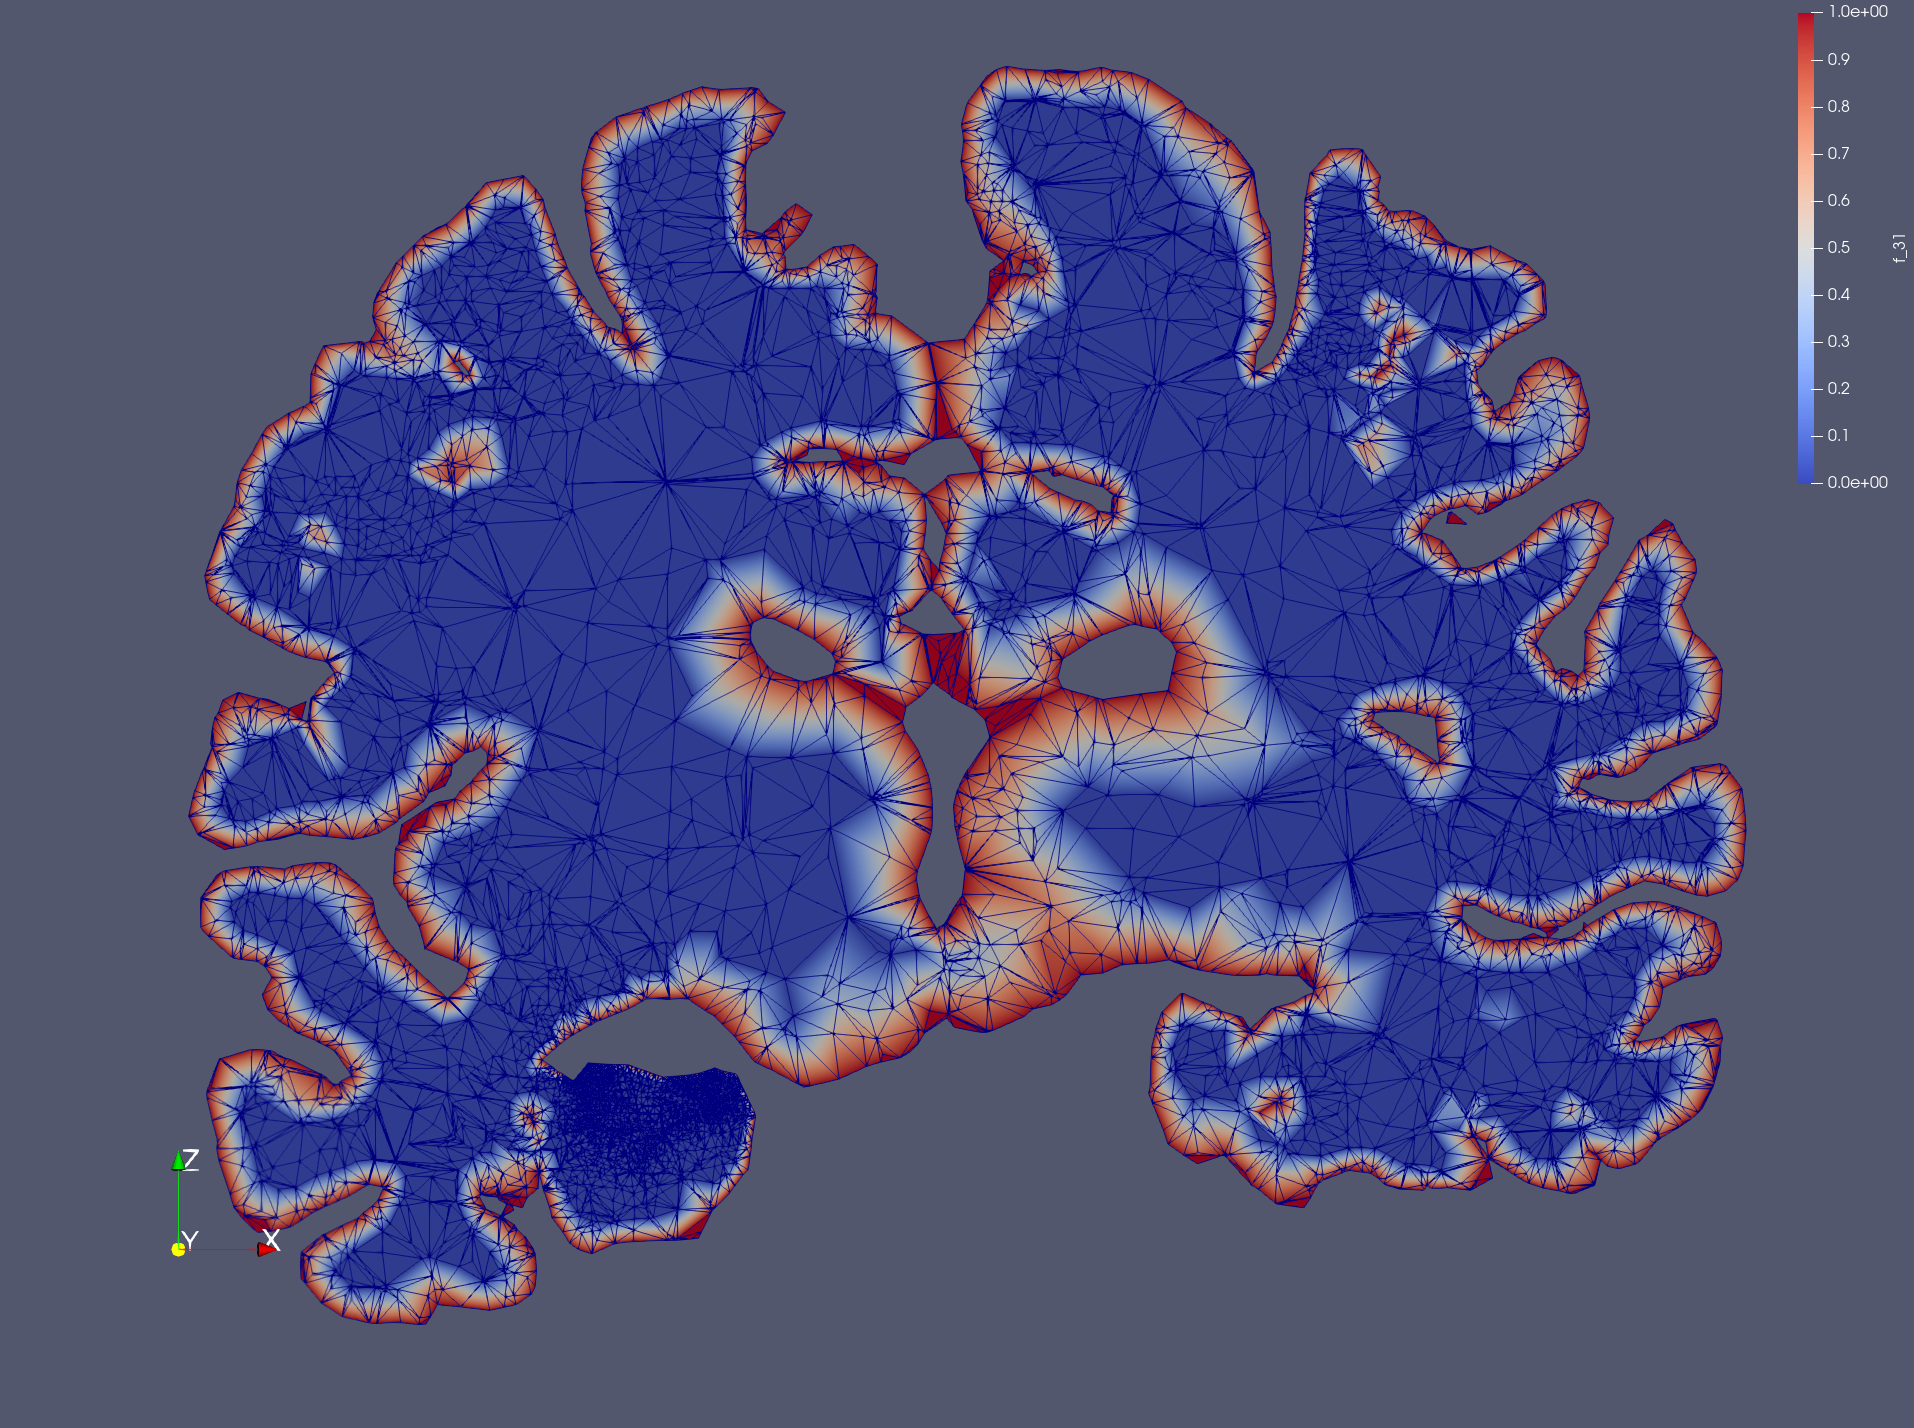
\includegraphics[width=0.49\textwidth]{./chapters/chp6/FIG/hippocampus_ref3_initialtime.png}
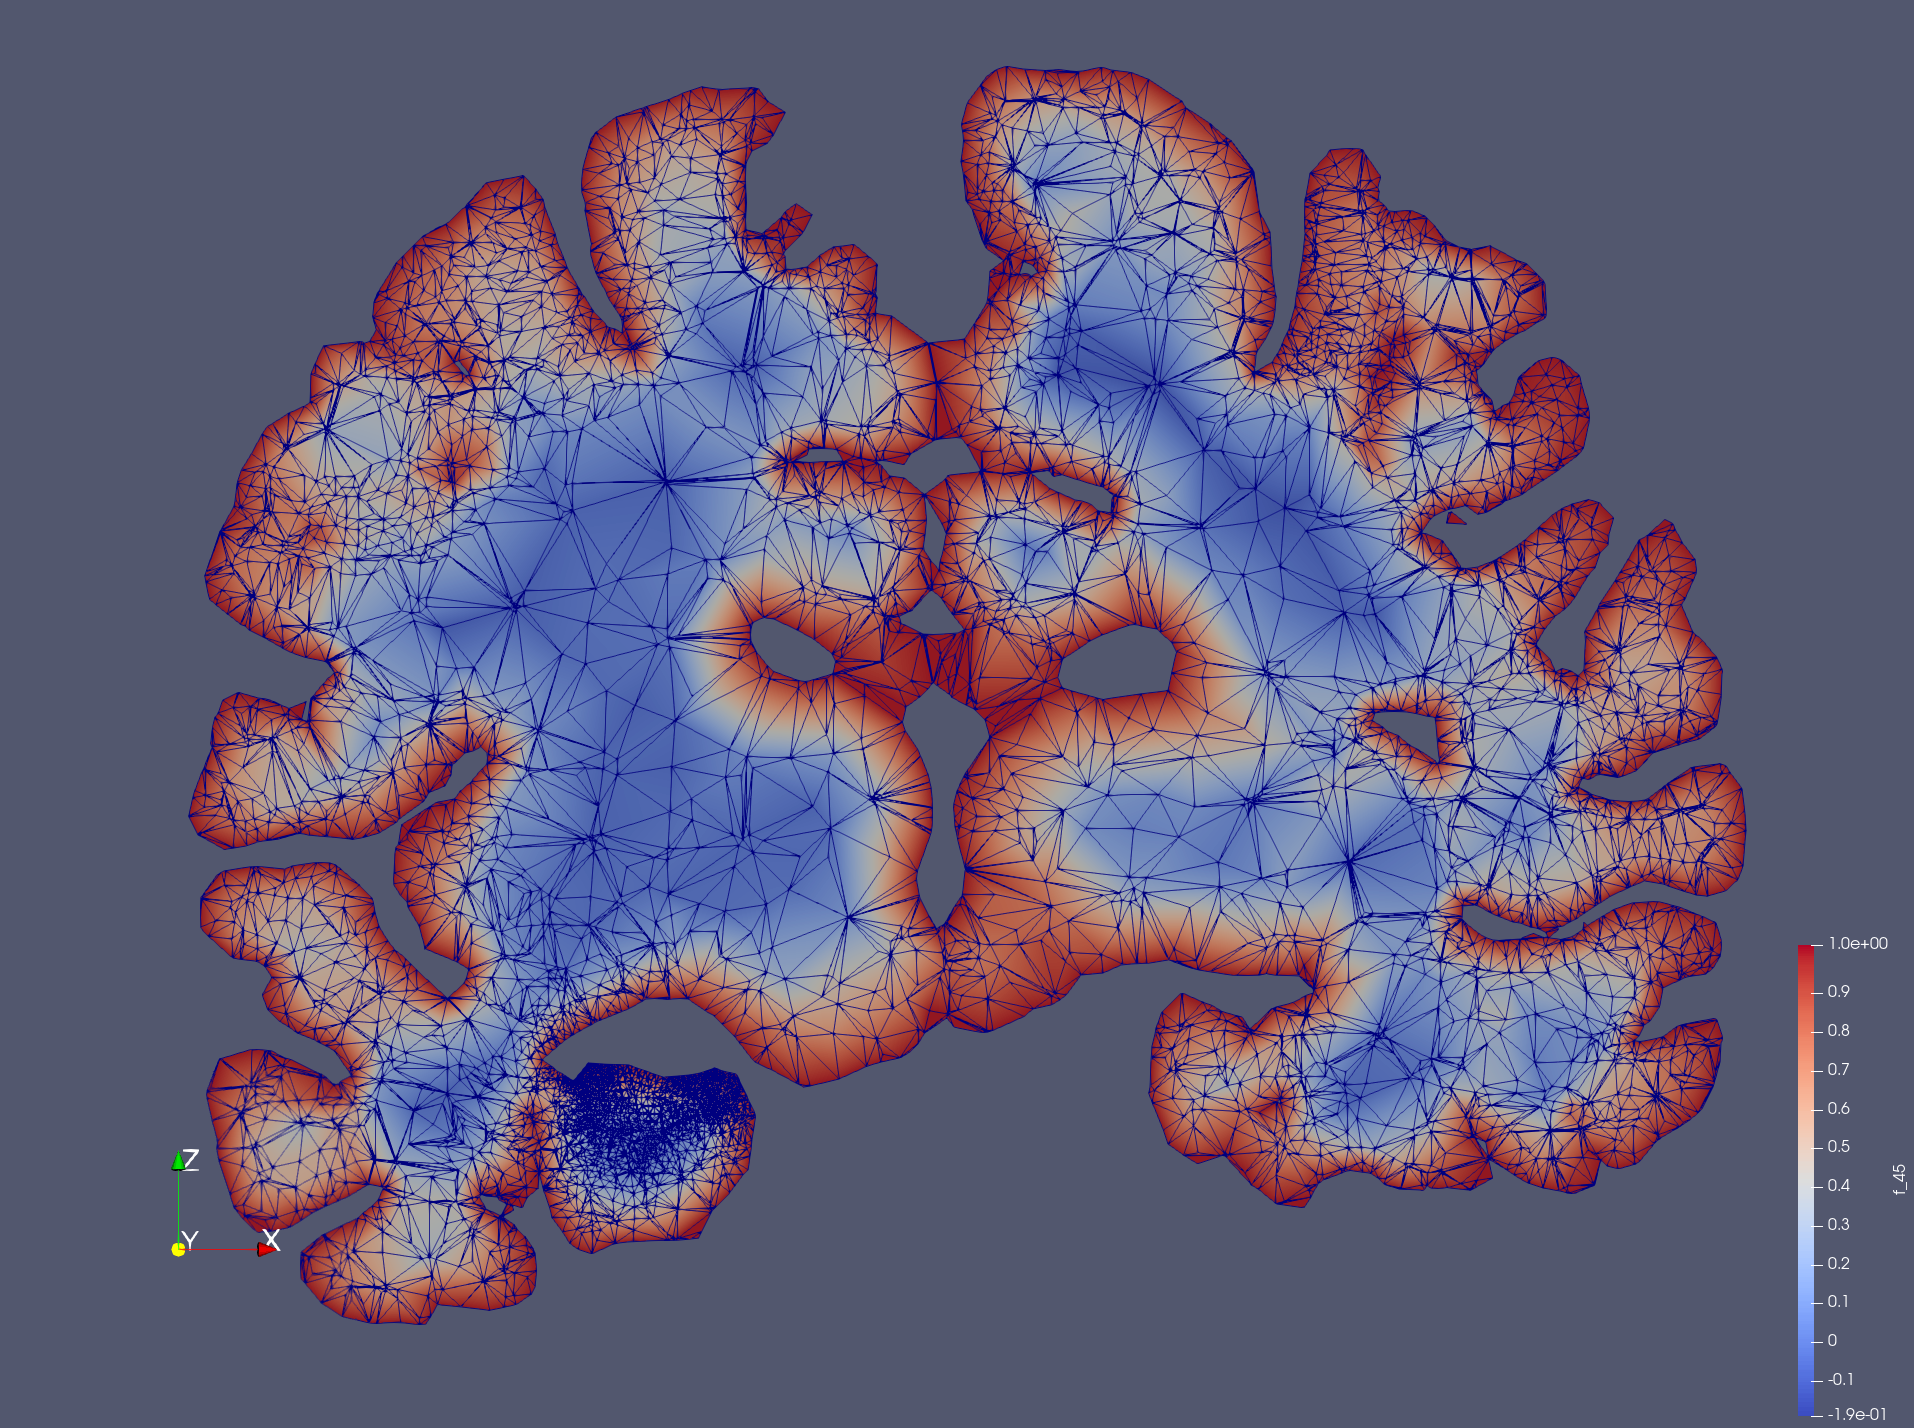
\includegraphics[width=0.49\textwidth]{./chapters/chp6/FIG/hippocampus_ref3_finaltime.png}
\caption{
%Distribution of Amyloid-beta over 5 mm in hippocampus during 9 hours with time step of 6 minutes are shown in the left 
%and right figure, respectively, when using local refinement in the hippocampus area.  
%The leftmost picture shows the initial distribution, while the rightmost image shows the 
%distribution after 9 hours. 
Distribution of Amyloid-beta over a 5mm hippocampal slice over a 9 hour time course; 
$\Delta t = 6/540$, adaptive hippocampal regional refinement. Initial concentration 
distribution (left) and final distribution (right). 
}
\label{fig:chp6:numerics4}
\end{figure}




\begin{table}%
  \label{chp6:meshstat}
  \centering
  \begin{minipage}{.45\textwidth}%
    \begin{tabular}{l|cccc}
	    Refinement & vertices & cells     & $h_{min}$ & $h_{max}$ \\ \hline
	     16 & 94K & 457K & 0.97 & 11.4 \\  
	     32 & 194K & 908K &  0.46 & 5.7 \\  
	     64 & 567K &  2.75M & 0.26 & 2.9 \\
	     128 &  2.8M & 15.5M &  0.14 & 1.45

    \end{tabular}
    %\caption{The number of vertices, cells and minimal and maximal mesh size of the uniformly refined meshes.}
    \caption{Mesh statistics, uniformly refined meshes of Figure~\ref{fig:chp6:numerics2}.}
    \label{tab:uniref}
  \end{minipage}%
    \qquad
  \begin{minipage}{.45\textwidth}%
    \begin{tabular}{c|cccc}
	    Refinement & vertices & cells     & $h_{min}$ & $h_{max}$ \\ \hline
	     1 & 99K &  479K &  0.64 &  11.4 \\
	     2 & 123K& 613K & 0.30 &  11.4 \\
	     3 & 275K &  1.5M  &  0.14 & 11.4 \\
	     4 & 1.3M &  7.7M  & 0.07 &  11.4 \\
    \end{tabular}
    %\caption{The number of vertices, cells and minimal and maximal mesh size of the locally refined meshes.}
    \caption{Mesh statistics, adaptively refined meshes of Figure~\ref{fig:chp6:numerics3}.}
    \label{tab:localref}
  \end{minipage}%
  \qquad

\end{table}

%\kent{
%Text left over from earlier
%}
%% \section{A closing perspective} 
%% In practice, an understanding of the flow of interstitial fluids through the 
%% brain is a critical question of interest for healthy brain function and metabolism;  
%% these questions lie at the heart of the removal of metabolic wastes, such as 
%% amyloid-beta or carbon dioxide, and the delivery of nutrition and oxygen to the 
%% many neuronal and glial cells of the parenchyma.  Numerous mathematical models 
%% have been used in the study of such questions.  Diffusion models were established 
%% in the seminal works of Nicolson\& Sykov{\'a} \cite{sykova2008diffusion} where 
%% well-crafted experiments, with molecules of different sizes, demonstrated that 
%% transport governed by extracellular diffusion is fundamental in the brain's metabolism. 
%% Further studies have examined to what extent convection may play a role in such 
%% models, in particular for larger molecules; for instance, convection enhanced 
%% delivery, by enforcing transmantle pressure gradients, has been proposed as method 
%% to accelerate the transport of drugs~\cite{bobo1994convection,stoverud2012modeling,kim2009voxelized} 
%% by pressurizing a region via infusion.  A separate model, such 
%% as Biot's equations or Darcy's equation, is often coupled to a tracer model, 
%% i.e.~a model similar to \eqref{eqn:chp6:model-problem}, which determines an interstitial fluid 
%% velocity, $\tnsr{z}(x,t) = -\tnsr{\kappa}(x)\Grad p$, where $\kappa(x)$ is a material 
%% permeability tensor and $p$ is the interstitial fluid pore pressure. 
%% The equation \eqref{eqn:chp6:model-problem} is then augmented by 
%% \begin{equation}\label{eqn:chp6:extended-model}
%% \partial_t u + \nabla\cdot(\tnsr{z} u) - \Div\left(\tnsr{K(x)} \Grad u\right) = f.
%% \end{equation} 
%% It is interesting to note that, in the computational drug transport studies 
%% \cite{stoverud2012modeling,kim2009voxelized}, the variations 
%% in permeability, informing $\tnsr{z}$, are larger than those of the molecular 
%% diffusivity tensor $\tnsr{K}$.  In this book, we have used the simpler version 
%% of the above model, i.e.~equation \eqref{eqn:chp6:model-problem}, as a prototype.  

%% The clinical perspective on waste and metabolite transport in the brain is 
%% changing.  Recently, it has been proposed that the cerebrospinal fluid plays an 
%% important role in the clearance of metabolic waste. The intimate coupling between 
%% the cerebrospinal fluid and the interstitial fluid, of the extracellular space, has 
%% been named the ``glymphatic system'' and is also referred to as the glymphatic 
%% hypothesis \cite{jessen2015glymphatic,iliff2012paravascular,xie2013sleep}.  It is 
%% critical, to the glymphatic theory, that this system facilitate convection; i.e.~that 
%% a model of glymphatic waste/metabolite/tracer transport model should include a term of the form 
%% $\nabla\cdot(\tnsr{z} u)$. While there have been studies of this type of system 
%% on the micro-level~\cite{holter2017interstitial,smith2018glymphatic}, simulations 
%% for the macroscopic behaviour of the such a system have not received much attention. 

%% New software is needed in order to thoroughly investigate leading clinical 
%% theories surrounding the clearance of waste material, or drug delivery, in the brain.  
%% In particular, a major reason for the current deficit is a lack of readily-accessible 
%% software to easily create the realistic, or patient-specific, 
%% computational prerequisites necessary for solving complex mathematical models.  
%% Mathematical models of porous flow, which can be coupled to equations such as 
%% \eqref{eqn:chp6:model-problem} or \eqref{eqn:chp6:extended-model}, are readily available; these include, for instance, 
%% Biot's equations \cite{goriely2015mechanics} or the equations of generalized 
%% poroelasticity \cite{chou2016fully, lee2019mixed}.  Conversely, before these 
%% models can even be solved, one needs to create high-quality meshes, with plausible 
%% realism, in a reasonable time-frame.  This text is aimed specifically at addressing 
%% the latter practical challenge.  We have shown how, beginning from a basic set of T1, T2, 
%% and diffusion patient MRI scans, one can systematically:  construct a computational 
%% volume mesh of the brain; mark subdomains and remove volumes; parcellate a volume mesh 
%% according to anatomical regions; create mesh subdomains based on parcellations; extract 
%% a diffusion tensor from dMRI data; and put everything together to solve a simple 
%% numerical model of tracer transport.  To accomplish this, we have provided the 
%% SVMTK software toolkit, and demonstrated its use alongside the open-source FEniCS 
%% numerical finite element library; thus enabling a new generation of computational 
%% studies for the investigation of important clinical theories. 




%% %the flow of interestitial fluids through the brain, which is 
%% %crucial for a healthy metabolism; i.e., the timely delivery of nutrition and oxygen as well as the 
%% %corresponding removal of metabolic waste and carbon dioxide, is often studied from the view point of either
%% %diffusion or porous media models. Diffusion models were established in the seminal works
%% %of Nicolson\& Sykov{\'a} \cite{sykova2008diffusion} where well crafted experiments with
%% %molecules of different sizes demonstrated that transport governed by extracellular diffusion is fundamental
%% %in the brain's metabolism. Later, several studies have examined to what extent convection may play a role, in
%% %particular for larger molecules. 
%% %For instance, convection enhanced delivery by enforcing transmantle pressure gradients has been proposed as method to 
%% %accelerate the transport of for instance drugs~\cite{bobo1994convection} by pressurizing a region by infusion. 
%% %Corresponding computational modeling studies are e.g.~\cite{stoverud2012modeling, kim2009voxelized}.    
%% %It is interesting to note that in these studies the variations in permeability are larger than that of diffusivity.
%% % 
%% %Recently, it has been proposed that the CSF plays an important role in the clearance of metabolic waste. The
%% %intimate coupling between the CSF and the interstitial fluid of the extracellular space has been named
%% %the glymphatic system~\cite{jessen2015glymphatic,iliff2012paravascular,xie2013sleep} and 
%% %it is crucial here that this system facilitate convection. While there has
%% %been many studies of this system on the micro-level~\cite{holter2017interstitial,smith2018glymphatic} 
%% %the macroscopic behaviour of the system has not received that much attention. 
%% %Part of the reason for this, we assume, is the lack of utilities to create patient-specific computational models easily. 
%% %While mathematical models for porous flow, such as 
%% %Biot's equations \cite{goriely2015mechanics} or the % 
%% %equations of generalized poroelasticity \cite{chou2016fully, lee2019mixed} are readily available, a crucial
%% %challenge is to create meshes with plausible realism in a reasonable time-frame. 
%% %\kent{We should mention several other studies, Eleonora, Ruiz-Baier.}



